\documentclass[11pt,a4paper]{article}

\usepackage[margin=2.3cm]{geometry}
\usepackage[T1]{fontenc}
\usepackage{lmodern}
\usepackage{microtype}
\usepackage{amsmath,amssymb,bm}
\usepackage{graphicx}
\usepackage{booktabs}
\usepackage{caption}
\usepackage{float}
\usepackage{xcolor}
\usepackage[colorlinks=true,linkcolor=blue!60!black,citecolor=blue!60!black,urlcolor=blue!60!black]{hyperref}

\graphicspath{{../crlb/crlb_results/}{../estimator/hybrid_map_results/}}

\newcommand{\vect}[1]{\bm{#1}}
\newcommand{\T}{\mathsf{T}}
\renewcommand{\H}{\mathsf{H}}
\newcommand{\udot}{\dot{\vect{u}}}
\newcommand{\pdot}{\dot{\vect{p}}}
\renewcommand{\Re}{\operatorname{Re}}
\renewcommand{\Im}{\operatorname{Im}}
\DeclareMathOperator{\tr}{tr}
\DeclareMathOperator{\rank}{rank}

\title{\textbf{Localization and Synchronization of a Mobile User\\
Aided by Reconfigurable Intelligent Surfaces\\ with Uncertain Positions}\\[0.6em]
\large B.Sc. Project Report --- English Summary}
\author{Mohammad Amin Khoshkam\\[0.3em]
\small Department of Electrical Engineering, Sharif University of Technology, Tehran, Iran\\[0.6em]
\small Supervisor: Dr.\ Rouhollah Amiri \qquad Project course instructor: Dr.\ Bijan Vosoughi Vahdat}
\date{\small Bahman 1404 (Winter 2026)}

\begin{document}
\maketitle

\begin{center}
\fbox{\parbox{0.92\linewidth}{\small
This document is a condensed English version of the original B.Sc.\ report, which was written in
Persian. It keeps the problem formulation, the main equations, the
numerical results and the conclusions; derivation details and the glossary are omitted.
All numbers are taken from the CSV outputs in \texttt{crlb/crlb\_results/} and
\texttt{estimator/hybrid\_map\_results/}.}}
\end{center}

\begin{abstract}
We jointly estimate the 3-D position and velocity of a mobile user equipment (UE), the relative frequency
error and the clock offset, and the positions, velocities and complex path gains associated with
reconfigurable intelligent surfaces (RISs). The base-station (BS) position is known, while the RIS geometry is
available only through a Gaussian prior; instead of assuming perfectly known RISs, the geometric uncertainty is
built directly into the localization, synchronization and estimation problem. The BS transmits OFDM pilots over
several subcarriers and time snapshots, and the received-signal model gathers time-varying delay, Doppler,
frequency error and clock offset into a single \emph{effective delay}. To obtain the fundamental accuracy limit,
the data information is combined with the RIS prior to form a hybrid Fisher information matrix (FIM); the
complex path gains are treated as nuisance parameters and removed with a Schur complement. We then propose a
hybrid maximum-a-posteriori / maximum-likelihood (MAP/ML) estimator in which only the RIS states use prior
information, while the UE, synchronization and channel parameters do not. Because the model is linear in the
path gains, these are eliminated analytically by variable projection; coarse-to-fine synchronization search,
random multi-start and local constrained optimization reduce sensitivity to initialization. With three RISs at
20~dB SNR, the position and velocity error bounds of the UE are 1.176~m and 1.864~m/s, and the bounds on the
frequency error and clock offset are 0.00146~ppm and 0.985~ns. In a numerical run, the estimator reduces the UE
position error from 3.212~m to 0.617~m with a normalized data-fit cost of 0.999 per sample. The results show that
localization and synchronization accuracy depends strongly on the quality of the RIS prior, and that even with a
full-rank FIM a poor geometry can produce a large condition number and noticeably degrade accuracy.
\end{abstract}

\noindent\textbf{Keywords:} reconfigurable intelligent surface; hybrid Cram\'er--Rao bound; MAP estimation;
variable projection; joint localization and synchronization; geometric uncertainty.

\tableofcontents
\newpage

%======================================================================
\section{Introduction}
%======================================================================

\subsection{Problem statement}
RISs create controllable reflected paths that extend coverage and provide a better geometry for localization,
which is especially valuable when the line-of-sight (LoS) path between the BS and the UE is weak or blocked.
However, an RIS can act as a reliable \emph{geometric anchor} only if its position and motion are known
accurately. In practice, surveying and installation errors, structural displacement, vibration and calibration
errors mean that the effective RIS position --- and even its velocity --- differs from the nominal values.
Treating these quantities as perfectly known leads to over-optimistic models and biased estimates; treating them
as completely unknown increases the number of unknowns and may make the problem unidentifiable.

This project considers the middle ground. The BS position $\vect{q}\in\mathbb{R}^3$ is known. A mobile UE has an
initial position $\vect{u}_0$ and constant velocity $\udot$, both unknown. $K$ RISs have initial positions
$\vect{p}_{k,0}$ and velocities $\pdot_k$ that are not known exactly; their uncertainty is described by a
Gaussian prior. In addition, the relative frequency error $\eta$, the clock offset $\delta_c$ and the complex path
gains $\beta_k$ are unknown. The BS transmits known OFDM pilots on $N$ subcarriers over $L$ time snapshots:
multiple subcarriers carry delay information, while multiple snapshots reveal the changes caused by UE motion,
RIS motion and Doppler.

Two questions are addressed:
\begin{enumerate}
\item Given unknown channel gains and uncertain RIS geometry, what is the fundamental accuracy achievable for UE
position, velocity and synchronization? This is answered with the hybrid FIM and hybrid Cram\'er--Rao bound.
\item How can an estimator exploit the available RIS prior without imposing artificial priors on the UE,
synchronization and channel parameters? This leads to the hybrid MAP/ML estimator.
\end{enumerate}

\subsection{Technical challenges}
\begin{itemize}
\item The phase of each observation is a periodic, nonlinear function of the effective delay, so the cost
function has many local minima and a local optimizer may not converge from a poor initial point.
\item The frequency error and clock offset are coupled with propagation delay and motion: the clock offset acts
like an extra delay, while frequency error and relative motion both create time-dependent phase changes. A single
snapshot cannot separate them; multiple snapshots are required.
\item The model is linear in the path gains $\beta_k$ but nonlinear in the geometric and synchronization
parameters. Searching jointly over all of them increases the dimension of the nonlinear problem.
\item Adding RIS positions and velocities as unknowns without any prior can make the FIM rank-deficient; an
over-confident prior, on the other hand, underestimates the true installation uncertainty.
\item A full-rank FIM does not guarantee numerical stability: a very large condition number means that some
directions in parameter space carry very little information.
\end{itemize}

\subsection{Contributions}
\begin{enumerate}
\item A discrete OFDM signal model for the direct path and $K$ RIS paths, including UE motion, RIS motion,
propagation delay, Doppler, frequency error and clock offset.
\item A unified parameter vector (UE state, synchronization, RIS states, complex gains), with an explicit mapping
between its conceptual ordering and the storage order in the code.
\item The data FIM, with prior information added \emph{only} to the RIS position and velocity blocks, so that no
artificial prior is placed on UE, synchronization or channel parameters.
\item Elimination of the channel gains as nuisance parameters with a Schur complement, and derivation of the
position error bound (PEB), velocity error bound (VEB) and synchronization bounds.
\item A hybrid MAP/ML estimator that jointly uses the RIS prior and the observations.
\item Variable projection to remove the channel gains analytically from the nonlinear search.
\item Coarse-to-fine search over the synchronization parameters, random multi-start and local constrained
optimization to reduce sensitivity to initialization.
\item Numerical study of the bounds and the estimator, of the effect of RIS prior quality, and of the effect of
geometry on rank, condition number and achievable accuracy.
\end{enumerate}

\subsection{Assumptions and scope}
\begin{itemize}
\item UE and RIS motion follow a constant-velocity model over the observation window (acceleration neglected).
\item Paths are resolvable, and the complex path gains are constant over the observation block; pilots are
perfectly known, and the post-processing noise is circularly symmetric complex white Gaussian.
\item Inter-carrier interference (ICI) is neglected: the normalized frequency error and residual Doppler are
assumed small compared with the subcarrier spacing, so their main effect is captured by phase and effective
delay.
\item Prior information exists only for the RIS states. Because part of the parameter vector is random (with a
prior) and part is deterministic, the framework is \emph{hybrid} --- neither fully Bayesian nor fully classical.
\end{itemize}

%======================================================================
\section{System and Signal Model}
%======================================================================

\subsection{Geometry and motion}
Subcarrier indices are symmetric around the centre subcarrier, $\mathcal{N}=\{-\tfrac{N-1}{2},\dots,0,\dots,
\tfrac{N-1}{2}\}$ for odd $N$, and the snapshot times are centred around zero,
\begin{equation}
T_l=\Bigl(l-\frac{L+1}{2}\Bigr)T_s,\qquad l=1,\dots,L,
\end{equation}
where $T_s$ is the snapshot interval. Centring the time axis is not cosmetic: it reduces the numerical
correlation between initial position and velocity, so the two are better separated. With constant velocities,
\begin{equation}
\vect{u}_l=\vect{u}_0+\udot\,T_l,\qquad \vect{p}_{k,l}=\vect{p}_{k,0}+\pdot_k\,T_l,\quad k=1,\dots,K.
\end{equation}
Path $k=0$ is the direct BS--UE path; paths $k=1,\dots,K$ go from the BS to RIS $k$ and then to the UE. Each RIS
creates one effective reflected path; its internal array response and phase profile are absorbed into
$\beta_k$, so the focus stays on position, motion and synchronization.

\subsection{Delay and path rate}
The delays of the direct and reflected paths are
\begin{equation}
\tau_{l,0}=\frac{1}{c}\|\vect{u}_l-\vect{q}\|,\qquad
\tau_{l,k}=\frac{1}{c}\bigl(\|\vect{q}-\vect{p}_{k,l}\|+\|\vect{p}_{k,l}-\vect{u}_l\|\bigr),
\end{equation}
and, with the sign convention used in the implementation, the geometric path rates are
\begin{align}
\nu_{l,0}&=\frac{1}{c}\,\frac{\udot^{\T}(\vect{u}_l-\vect{q})}{\|\vect{u}_l-\vect{q}\|},\\
\nu_{l,k}&=\frac{1}{c}\left(-\frac{\pdot_k^{\T}(\vect{q}-\vect{p}_{k,l})}{\|\vect{q}-\vect{p}_{k,l}\|}
+\frac{(\pdot_k-\udot)^{\T}(\vect{p}_{k,l}-\vect{u}_l)}{\|\vect{p}_{k,l}-\vect{u}_l\|}\right).
\end{align}
Sign conventions for path rate and Doppler differ between references; what matters is that the definition of
$\nu_{l,k}$, the effective delay and the signal phase are consistent throughout the derivations and the code.

\subsection{Clock offset, frequency error and effective delay}
The UE and BS oscillators are related by $f_{\mathrm{UE}}=(1+\eta)f_{\mathrm{BS}}$, where $\eta$ is the
(dimensionless) relative frequency error, and $\delta_c$ is the clock offset between the two time references.
Linearizing the path variations over the observation window, all effects are gathered into one effective delay:
\begin{equation}
a_{l,k}=\tau_{l,k}-(\nu_{l,k}-\eta)\,T_l-\delta_c .
\label{eq:effdelay}
\end{equation}
The estimator never observes these effects separately but only through $a_{l,k}$; separating them requires
sufficient frequency \emph{and} time diversity. In the default \texttt{reference-linearized} geometry model,
$\tau_{l,k}$ and $\nu_{l,k}$ are evaluated at the reference time and motion enters through the $T_l$ term.

\subsection{Received signal}
After cyclic-prefix removal and the DFT, the sample on subcarrier $n$ in snapshot $l$ is
\begin{equation}
y_{n,l}=\sqrt{\frac{\varepsilon}{N}}\,x_{n,l}\sum_{k=0}^{K}\beta_k\exp\bigl(-j2\pi n\Delta f\,a_{l,k}\bigr)
+z_{n,l},\qquad z_{n,l}\sim\mathcal{CN}(0,\sigma^2),
\label{eq:rx}
\end{equation}
where $x_{n,l}$ is the known pilot, $\varepsilon$ the pilot energy and $\Delta f$ the subcarrier spacing.
Stacking all samples as $\vect{y}=\operatorname{vec}\{y_{n,l}\}\in\mathbb{C}^{NL}$ and defining the design
matrix $\vect{A}(\vect{\theta})\in\mathbb{C}^{NL\times(K+1)}$ with entries
\begin{equation}
[\vect{A}(\vect{\theta})]_{(n,l),k}=\sqrt{\varepsilon/N}\,x_{n,l}\exp\bigl(-j2\pi n\Delta f\,a_{l,k}(\vect{\theta})\bigr),
\end{equation}
the model becomes
\begin{equation}
\vect{y}=\vect{A}(\vect{\theta})\,\vect{\beta}+\vect{z},\qquad
\vect{\beta}=[\beta_0,\dots,\beta_K]^{\T}.
\label{eq:vector}
\end{equation}
Model~\eqref{eq:vector} is the key relation of the project: $\vect{A}$ depends nonlinearly on position, velocity
and synchronization, but the model is \emph{linear} in $\vect{\beta}$. For a fixed $\vect{\theta}$, the optimal
$\vect{\beta}$ can therefore be computed in closed form.

\subsection{Parameter vector}
The physical parameters are stored in the MATLAB code as
\begin{equation}
\vect{\theta}=\bigl[\vect{u}_0^{\T},\ \udot^{\T},\ \vect{p}_{1,0}^{\T},\dots,\vect{p}_{K,0}^{\T},\
\pdot_1^{\T},\dots,\pdot_K^{\T},\ \eta,\ \delta_c\bigr]^{\T}\in\mathbb{R}^{8+6K}.
\end{equation}
For the statistical analysis they are grouped by role: the UE and synchronization parameters
$\vect{\psi}=[\vect{u}_0^{\T},\udot^{\T},\eta,\delta_c]^{\T}\in\mathbb{R}^8$ (no prior) and the RIS states
$\vect{\rho}\in\mathbb{R}^{6K}$ (with prior), extracted with selection matrices $\vect{\psi}=\vect{E}_\psi\vect{\theta}$,
$\vect{\rho}=\vect{E}_\rho\vect{\theta}$. For a real-valued FIM, the complex gains are split into real and
imaginary parts,
\begin{equation}
\vect{\gamma}=\bigl[\vect{\theta}^{\T},\ \Re\{\vect{\beta}\}^{\T},\ \Im\{\vect{\beta}\}^{\T}\bigr]^{\T}\in\mathbb{R}^{10+8K}.
\end{equation}
For $K=3$: $\dim(\vect{\theta})=26$ and $\dim(\vect{\gamma})=34$.

%======================================================================
\section{Hybrid Fisher Information and Estimation Bounds}
%======================================================================

\subsection{Data information}
The noiseless mean is $\vect{\mu}(\vect{\gamma})=\vect{A}(\vect{\theta})\vect{\beta}$. For complex white
Gaussian noise with covariance $\sigma^2\vect{I}$, the FIM entries are~\cite{kay1993}
\begin{equation}
[\vect{J}_{\mathrm{data}}]_{i,j}=\frac{2}{\sigma^2}\sum_{l=1}^{L}\sum_{n\in\mathcal{N}}
\Re\left\{\Bigl(\frac{\partial\mu_{n,l}}{\partial\gamma_i}\Bigr)^{*}\frac{\partial\mu_{n,l}}{\partial\gamma_j}\right\},
\end{equation}
with
\begin{equation}
\frac{\partial\mu_{n,l}}{\partial\theta_i}=\sqrt{\frac{\varepsilon}{N}}\,x_{n,l}\sum_{k=0}^{K}\beta_k
e^{-j2\pi n\Delta f a_{l,k}}\,(-j2\pi n\Delta f)\,\frac{\partial a_{l,k}}{\partial\theta_i},
\qquad \frac{\partial a_{l,k}}{\partial\eta}=T_l,\quad \frac{\partial a_{l,k}}{\partial\delta_c}=-1 .
\end{equation}
Geometric derivatives use $\nabla_{\vect{r}}\|\vect{r}\|=\vect{w}$ and
$\nabla_{\vect{r}}\vect{w}=\vect{P}^{\perp}_{\vect{w}}/d$ with $\vect{w}=\vect{r}/\|\vect{r}\|$,
$\vect{P}^{\perp}_{\vect{w}}=\vect{I}-\vect{w}\vect{w}^{\T}$. In the implementation, position and velocity
derivatives are computed with central finite differences and checked against simpler analytic relations to avoid
sign errors in long expressions.

\subsection{RIS prior and the hybrid FIM}
The RIS states follow $\vect{\rho}\sim\mathcal{N}(\bar{\vect{\rho}},\vect{Q}^{-1})$ with the isotropic precision
\begin{equation}
\vect{Q}=\operatorname{blkdiag}\Bigl(\tfrac{1}{\sigma_p^2}\vect{I}_{3K},\ \tfrac{1}{\sigma_v^2}\vect{I}_{3K}\Bigr),
\qquad \vect{J}_{\mathrm{prior},\theta}=\vect{E}_\rho^{\T}\vect{Q}\vect{E}_\rho,
\end{equation}
and the hybrid FIM is $\vect{J}_\gamma=\vect{J}_{\mathrm{data}}+\vect{J}_{\mathrm{prior}}$, where the prior blocks
for UE, synchronization and channel parameters are zero.

Three cases must be distinguished: a parameter that is \emph{exactly known} is not part of the unknown vector; a
parameter that is \emph{uncertain but has a prior} must stay in the vector with its prior added (dropping it would
hide its effect on the UE estimate and yield an over-optimistic bound); and a pure \emph{nuisance} parameter must
be removed with a Schur complement, not by deleting its row and column. Here only the channel gains are nuisance
parameters.

\subsection{Removing the channel gains}
Partitioning $\vect{J}_\gamma$ into the physical block and the block of $\vect{b}=[\Re\{\vect{\beta}\}^{\T},
\Im\{\vect{\beta}\}^{\T}]^{\T}$, the equivalent information on the physical parameters is
\begin{equation}
\vect{J}_e=\vect{J}_{\theta\theta}-\vect{J}_{\theta b}\vect{J}_{bb}^{\dagger}\vect{J}_{b\theta}.
\end{equation}
Using $\vect{J}_{\theta\theta}$ alone would amount to assuming known channel gains and would give an
over-optimistic bound.

\subsection{Reported bounds}
If $\vect{J}_e$ is full rank, any locally unbiased estimator satisfies $\vect{C}_\theta\succeq\vect{J}_e^{-1}$,
and the reported metrics are
\begin{equation}
\mathrm{PEB}_{\mathrm{UE}}=\sqrt{\tr\bigl([\vect{C}_\theta]_{\vect{u}_0,\vect{u}_0}\bigr)},\quad
\mathrm{VEB}_{\mathrm{UE}}=\sqrt{\tr\bigl([\vect{C}_\theta]_{\udot,\udot}\bigr)},\quad
\sigma_{\eta,\mathrm{LB}}=\sqrt{[\vect{C}_\theta]_{\eta,\eta}},\quad
\sigma_{\delta,\mathrm{LB}}=\sqrt{[\vect{C}_\theta]_{\delta_c,\delta_c}},
\end{equation}
with analogous $\mathrm{PEB}_{\mathrm{RIS},k}$ and $\mathrm{VEB}_{\mathrm{RIS},k}$. The frequency-error bound is
reported in ppm ($\times10^6$) and the clock-offset bound in ns ($\times10^9$).

\subsection{Rank, identifiability and condition number}
Local identifiability of all physical parameters requires $\rank(\vect{J}_e)=8+6K$. A pseudoinverse keeps the
computation running in the rank-deficient case but creates no information that is not in the data. Even with full
rank, the condition number $\kappa(\vect{J}_e)=\lambda_{\max}/\lambda_{\min}$ must be checked: a large value means
some directions carry far less information than others, making the problem sensitive to noise, scaling and the
starting point.

%======================================================================
\section{Hybrid MAP/ML Estimator}
%======================================================================

\subsection{Joint cost function}
$\vect{\psi}$ and $\vect{\beta}$ are deterministic unknowns estimated by ML; $\vect{\rho}$ has a prior and is
estimated by MAP. With the likelihood $p(\vect{y}\mid\vect{\theta},\vect{\beta})\propto
\exp(-\|\vect{y}-\vect{A}(\vect{\theta})\vect{\beta}\|_2^2/\sigma^2)$ and the Gaussian prior on $\vect{\rho}$,
\begin{equation}
(\hat{\vect{\theta}},\hat{\vect{\beta}})=\arg\min_{\vect{\theta}\in\Theta,\ \vect{\beta}}
\left[\frac{\|\vect{y}-\vect{A}(\vect{\theta})\vect{\beta}\|_2^2}{\sigma^2}
+\frac{1}{2}(\vect{\rho}-\bar{\vect{\rho}})^{\T}\vect{Q}(\vect{\rho}-\bar{\vect{\rho}})\right],
\end{equation}
where $\Theta$ holds the physical constraints. The prior term must enter with a \emph{positive} sign (it comes
from the negative log of a Gaussian); a negative sign would reward distance from the prior mean and make the cost
unbounded below. In the limits, $\sigma_p,\sigma_v\to\infty$ gives a pure ML estimator, while
$\sigma_p,\sigma_v\to0$ pins the RISs to their prior mean.

\subsection{Variable projection}
For fixed $\vect{\theta}$, the gains solve a linear least-squares problem,
$\hat{\vect{\beta}}(\vect{\theta})=\vect{A}^{\dagger}(\vect{\theta})\vect{y}$ (computed with an SVD rather than
an explicit inverse). With $\vect{P}^{\perp}_{\vect{A}}=\vect{I}-\vect{A}\vect{A}^{\dagger}$, the concentrated
problem involves only the physical parameters~\cite{golub1973}:
\begin{equation}
\hat{\vect{\theta}}=\arg\min_{\vect{\theta}\in\Theta}J_c(\vect{\theta}),\qquad
J_c(\vect{\theta})=\frac{\|\vect{P}^{\perp}_{\vect{A}(\vect{\theta})}\vect{y}\|_2^2}{\sigma^2}
+\frac{1}{2}(\vect{\rho}-\bar{\vect{\rho}})^{\T}\vect{Q}(\vect{\rho}-\bar{\vect{\rho}}).
\end{equation}
For $K=3$ this removes four complex gains (eight real variables) from the nonlinear search. The
$NL\times NL$ projector is never formed: the residual is computed as $\vect{r}=\vect{y}-\vect{A}\hat{\vect{\beta}}$,
which matters for $NL=4128$. Using $\vect{A}^{\H}\vect{r}=\vect{0}$, the gradient is
\begin{equation}
\nabla_{\theta}J_c=-\frac{2}{\sigma^2}\Re\{\vect{D}_\theta^{\H}\vect{r}\}+\vect{E}_\rho^{\T}\vect{Q}(\vect{\rho}-\bar{\vect{\rho}}),
\qquad \vect{D}_\theta=\frac{\partial[\vect{A}(\vect{\theta})\hat{\vect{\beta}}(\vect{\theta})]}{\partial\vect{\theta}^{\T}},
\end{equation}
with finite-difference steps of $10^{-3}$~m for positions and $10^{-2}$~m/s for velocities.

\subsection{Scaling and constraints}
Parameters differ by many orders of magnitude (metres, m/s, $\eta\sim10^{-6}$, $\delta_c\sim10^{-9}$~s), so the
optimizer works on scaled variables with $\vect{S}=\operatorname{diag}(1,\dots,1,10^{-6},10^{-9})$. Global bounds
are $[0,25]$~m for the horizontal UE position, $[0,10]$~m for height, $[-5,5]$~m/s for velocity components,
$[-20,20]$~ppm for $\eta$ and $[-300,300]$~ns for $\delta_c$. Around each starting point a local box is added to
keep the solver away from distant periodic solutions; an active local bound in the final solution indicates that
the box may be too small.

\subsection{Initialization and optimization}
Much of the multimodality comes from $\eta$ and $\delta_c$, so they are initialized in two stages: a coarse grid
of $25\times33$ points over $(\eta,\delta_c)$, then a $13\times13$ local grid around the best coarse point. At
every grid point the gains are re-estimated by least squares, so points are compared at their best possible
channel fit. The full algorithm is:
\begin{enumerate}
\item build $\vect{y}$, the centred times and the pilot matrix;
\item set the mean and precision of the RIS prior;
\item run the coarse and fine search over $(\eta,\delta_c)$ on the concentrated cost;
\item generate random starting points (Gaussian perturbations around the initial estimate), apply the
constraints and sort them by cost;
\item run a constrained SQP solver (\texttt{fmincon}) from the eight best points, with at most 600 iterations
and 30\,000 function evaluations each;
\item keep the solution with the lowest final cost and recover $\hat{\vect{\beta}}$;
\item compute the residual, check active local bounds, the FIM rank and the condition number.
\end{enumerate}
A useful diagnostic is the normalized residual $\|\vect{r}\|_2^2/(NL\sigma^2)$, which should be close to one for
a good fit; values well above one suggest model error or a poor local minimum, and values well below one suggest
over-estimated noise or over-fitting.

\subsection{Relation to the bound}
The bound is a local property of the statistical model and the scenario, while the estimator is an algorithm run on
one noise realization. Comparing the estimator with the bound therefore requires many Monte Carlo runs under
identical settings; the local bound at the estimate is useful for spotting weak directions but does not replace
an RMSE-vs-CRLB comparison.

%======================================================================
\section{Simulation Results}
%======================================================================

\subsection{Common settings}
Two independent sets of outputs were produced: one for the hybrid bound and one for the hybrid MAP/ML estimator.
They share the settings in Table~\ref{tab:settings}. The observation window spans $-77.5$ to $77.5$~ms and gives
$NL=4128$ complex samples. Pilots are unit-amplitude QPSK, the true path gains are
$\vect{\beta}=[0.98877+j0.14944,\ 0.45286-j0.46628,\ 0.08498+j0.49272,\ -0.23540-j0.32340]^{\T}$, and the random
seed is 42 in all runs.

\begin{table}[H]
\centering
\caption{Main simulation settings.}
\label{tab:settings}
\begin{tabular}{llll}
\toprule
Parameter & Value & Parameter & Value\\
\midrule
$K$ (RISs / reflected paths) & 3 & $\sigma_p$ (RIS position std, per axis) & 0.1 m\\
$N$ (subcarriers, $-64\dots64$) & 129 & $\sigma_v$ (RIS velocity std, per axis) & 0.05 m/s\\
$L$ (snapshots) & 32 & $\eta$ (true) & 2 ppm\\
$\Delta f$ & 480 kHz & $\delta_c$ (true) & 40 ns\\
$T_s$ & 5 ms & Geometry model & reference-linearized\\
SNR (default) & 20 dB & & \\
\bottomrule
\end{tabular}
\end{table}

\paragraph{The two scenarios differ.} The bound uses $\vect{q}=[0,0,5]^{\T}$~m and $\vect{u}_0=[8,7,1.5]^{\T}$~m,
while the estimator uses $\vect{q}=[3,4,5]^{\T}$~m and $\vect{u}_0=[8,10,1.5]^{\T}$~m. In both, the RISs are at
$(0,18,3)$, $(20,0,4)$ and $(18,18,6)$~m with zero velocity. Because the CRLB depends strongly on geometry, the
estimator error is \emph{not} plotted on the bound curve of the other scenario; each set is analysed in its own
geometry, and the estimator is compared only with the local bound saved in the same run.

\subsection{Hybrid bound results}

\begin{figure}[H]
\centering
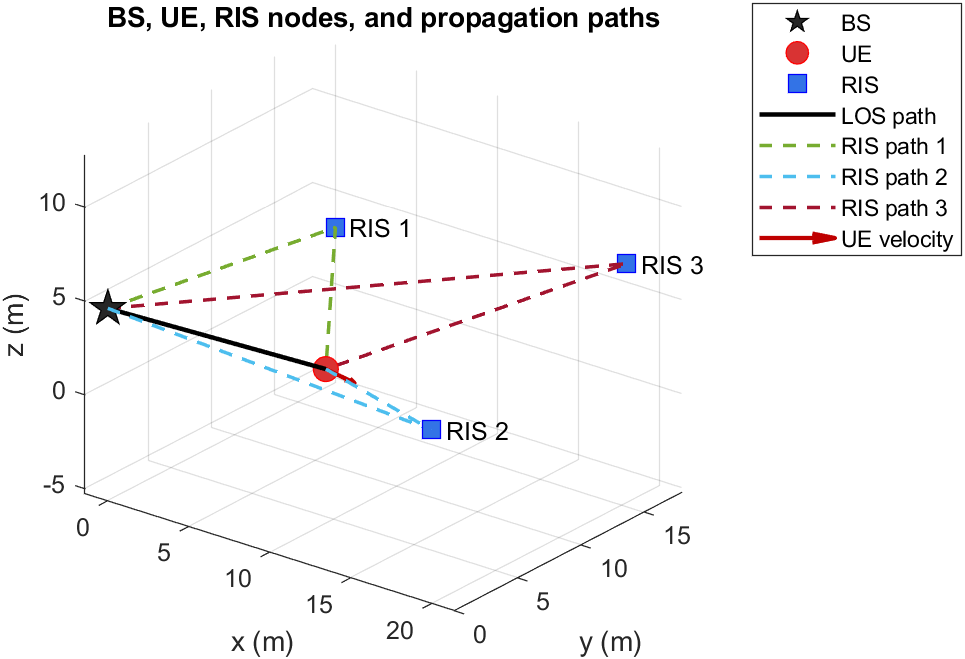
\includegraphics[width=0.62\linewidth]{01_geometry.png}
\caption{Geometry of the BS, the UE and the three RISs in the bound scenario. Solid line: direct path; dashed
lines: RIS paths.}
\label{fig:geom}
\end{figure}

The three RISs lie in different directions from the UE and provide good diversity in the horizontal plane, while
height differences are small and give little diversity in the vertical direction
(Fig.~\ref{fig:geom}). As shown next, this makes the $z$-axis parameters harder to estimate.

\begin{figure}[H]
\centering
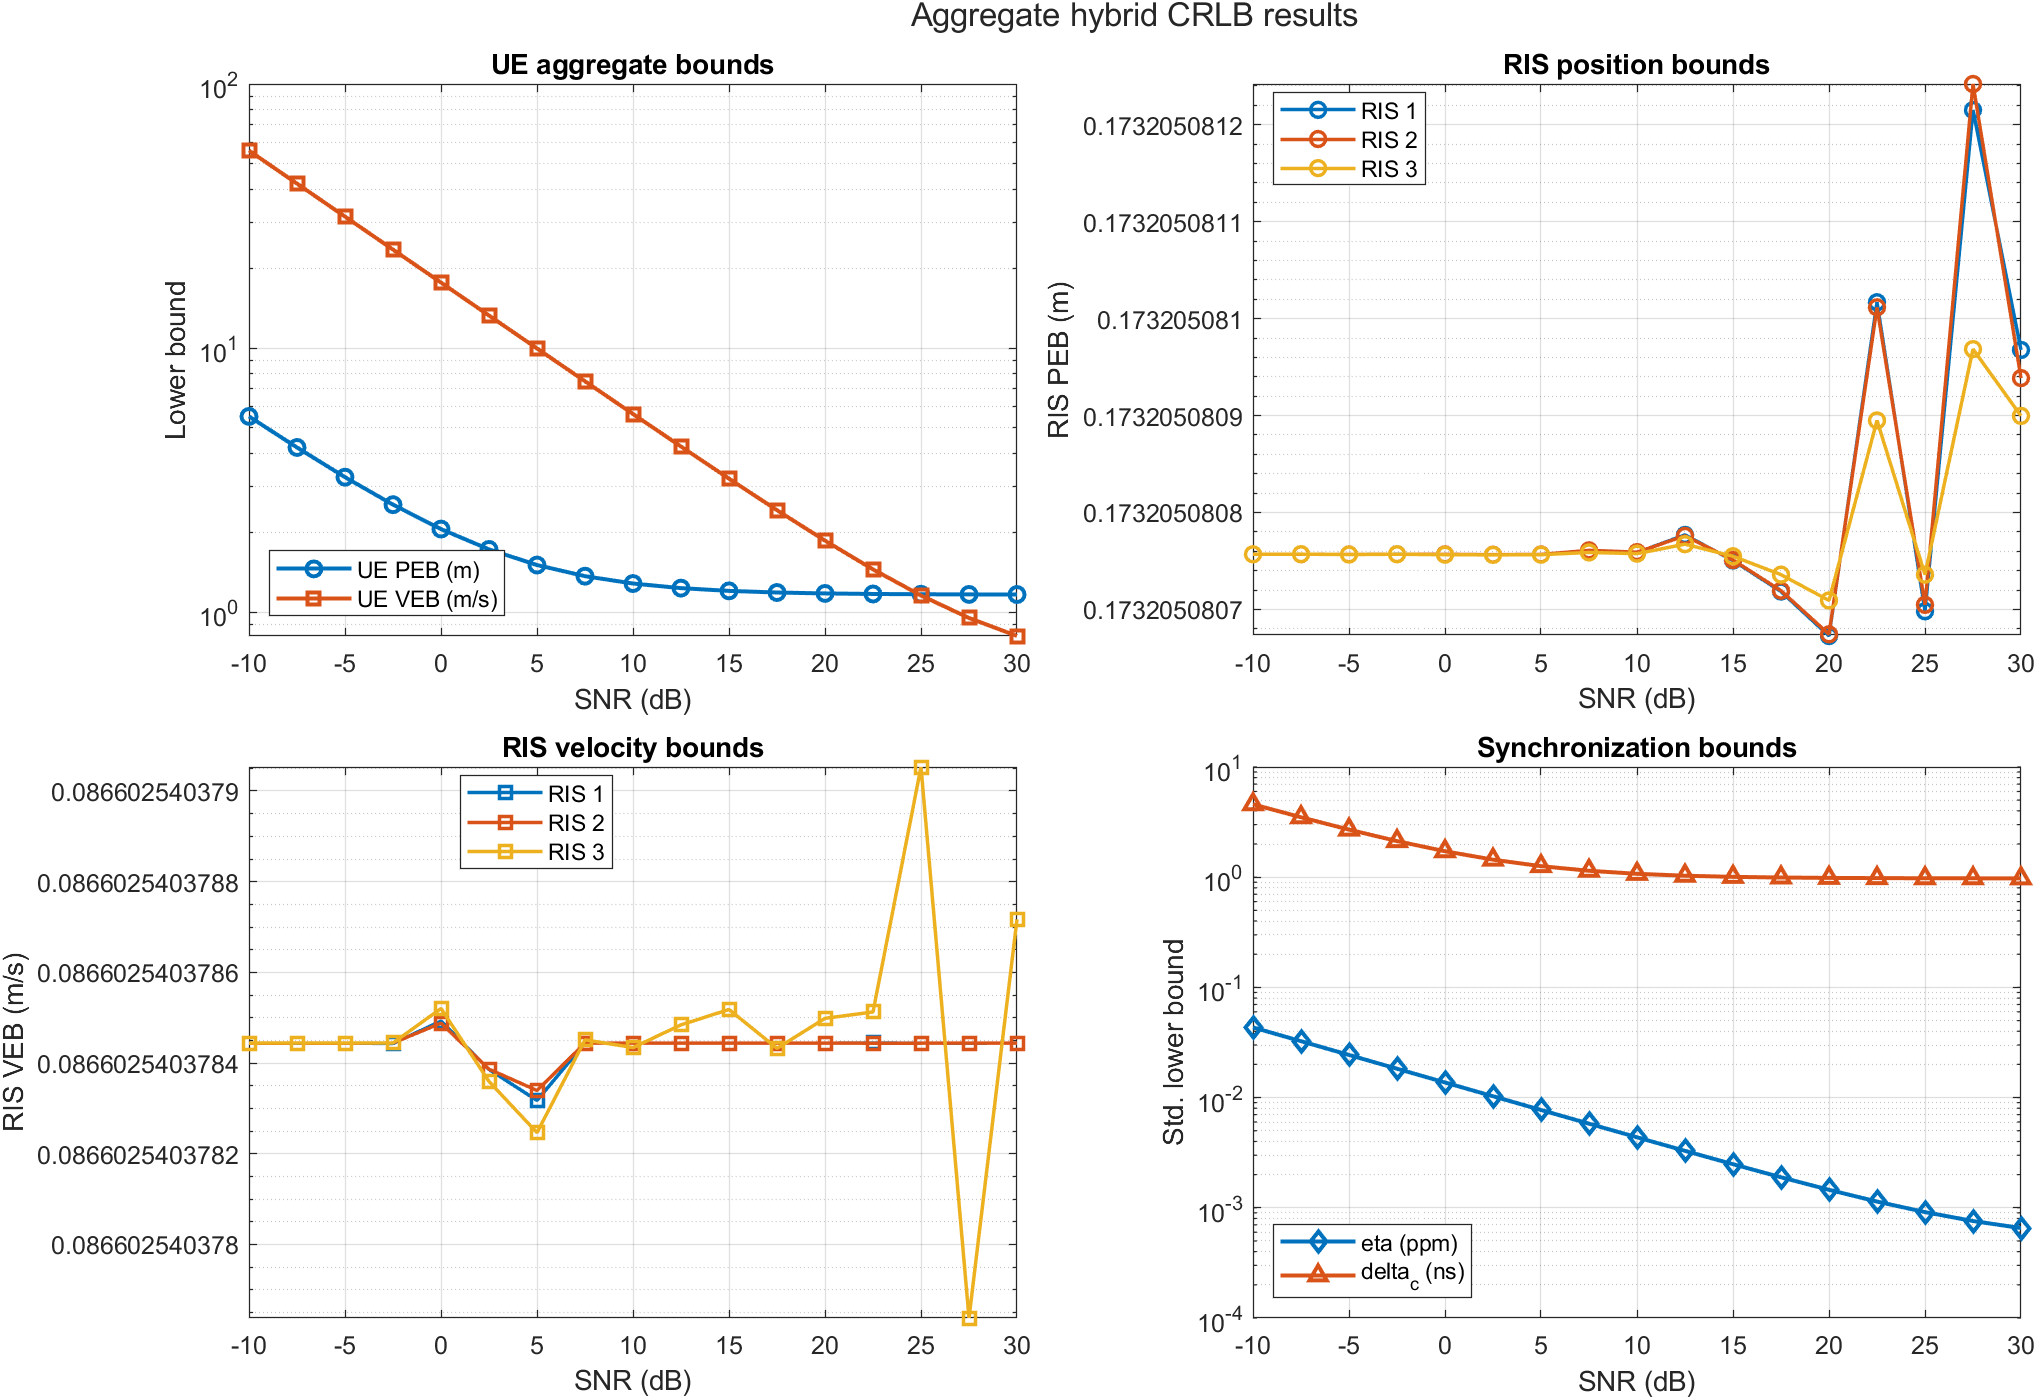
\includegraphics[width=0.95\linewidth]{02_main_bounds.png}
\caption{Aggregate bounds of the UE, the RISs and the synchronization parameters versus SNR.}
\label{fig:snr}
\end{figure}

\paragraph{Bounds versus SNR.} Over $-10$ to $30$~dB (Fig.~\ref{fig:snr}), the UE PEB falls from 5.506~m to
1.165~m but flattens to an \emph{error floor} of about 1.16~m at high SNR; the clock-offset bound similarly falls
from 4.586~ns to about 0.976~ns and saturates. In contrast, the UE VEB (55.94 to 0.811~m/s) and the $\eta$ bound
(0.04334 to 0.000655~ppm) keep decreasing. Time diversity from many snapshots is very effective for rate-type
parameters, whereas for some position and timing parameters the RIS geometric uncertainty and the coupling
between delays prevent unlimited improvement with more power. The tiny fluctuations of the RIS curves (order
$10^{-9}$--$10^{-8}$) are numerical, not physical.

\begin{table}[H]
\centering
\caption{Hybrid bounds at SNR = 20 dB (\texttt{summary\_bounds.csv}).}
\label{tab:bounds}
\begin{tabular}{lrl}
\toprule
Quantity & Bound (std / vector error) & Unit\\
\midrule
UE position (PEB) & 1.17623 & m\\
UE velocity (VEB) & 1.86396 & m/s\\
Position of each RIS & 0.173205 & m\\
Velocity of each RIS & 0.086603 & m/s\\
Relative frequency error $\eta$ & 0.001456 & ppm\\
Clock offset $\delta_c$ & 0.985476 & ns\\
\bottomrule
\end{tabular}
\end{table}

The RIS position bound equals $\sqrt{3}\sigma_p=0.173205$~m and the RIS velocity bound equals
$\sqrt{3}\sigma_v=0.086603$~m/s (Table~\ref{tab:bounds}): in this configuration the observations are not enough
to noticeably reduce the RIS uncertainty, and the prior dominates these blocks.

\begin{figure}[H]
\centering
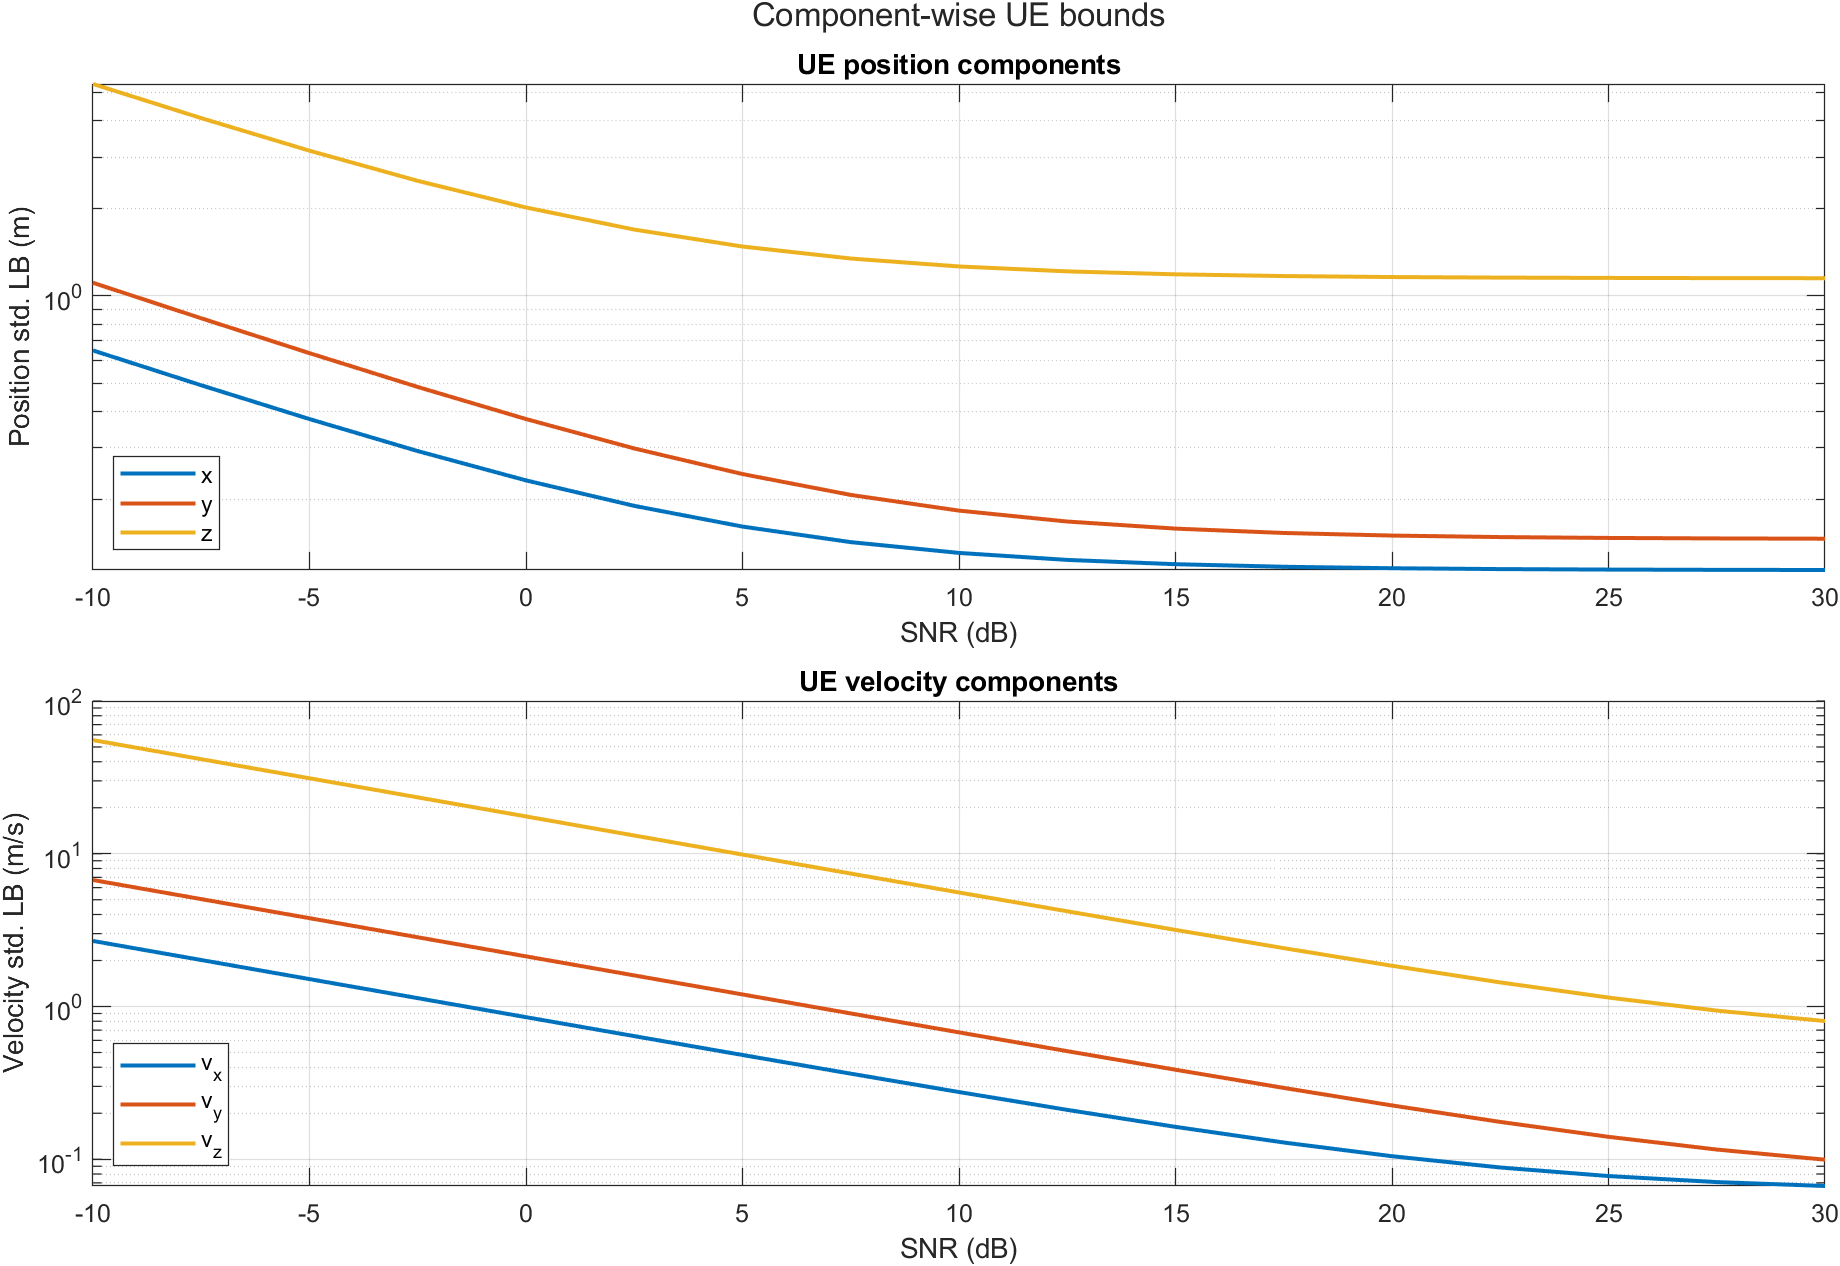
\includegraphics[width=0.85\linewidth]{03_ue_components.png}
\caption{Per-axis bounds of UE position and velocity.}
\label{fig:uecomp}
\end{figure}

\paragraph{Per-axis UE bounds.} At 20~dB the position bounds along $x,y,z$ are about 0.116, 0.150 and 1.161~m,
and the velocity bounds are about 0.105, 0.225 and 1.847~m/s (Fig.~\ref{fig:uecomp}). The PEB is therefore
dominated by the vertical axis --- a geometric property of the scenario that higher SNR alone cannot fix. Per-axis
RIS bounds stay at $\sigma_p=0.1$~m and $\sigma_v=0.05$~m/s and are almost flat in SNR. For the channel gains, the
imaginary-part bounds of the first two reflected paths (about 0.01195 and 0.01045 at 20~dB) are larger than
others: the same number of observations does not mean the same information about each path.

\paragraph{Rank and conditioning.} At the default point the equivalent physical FIM has rank 26/26 and the full
FIM rank 34/34, so no pseudoinverse was needed for rank deficiency. The condition number, however, is about
$9.25\times10^{7}$. The eigenvalue spread and the correlation structure (Fig.~\ref{fig:fim}) show strong coupling
among some geometric, timing and channel parameters, which is one of the main reasons the vertical UE component is
poorly estimated.

\begin{figure}[H]
\centering
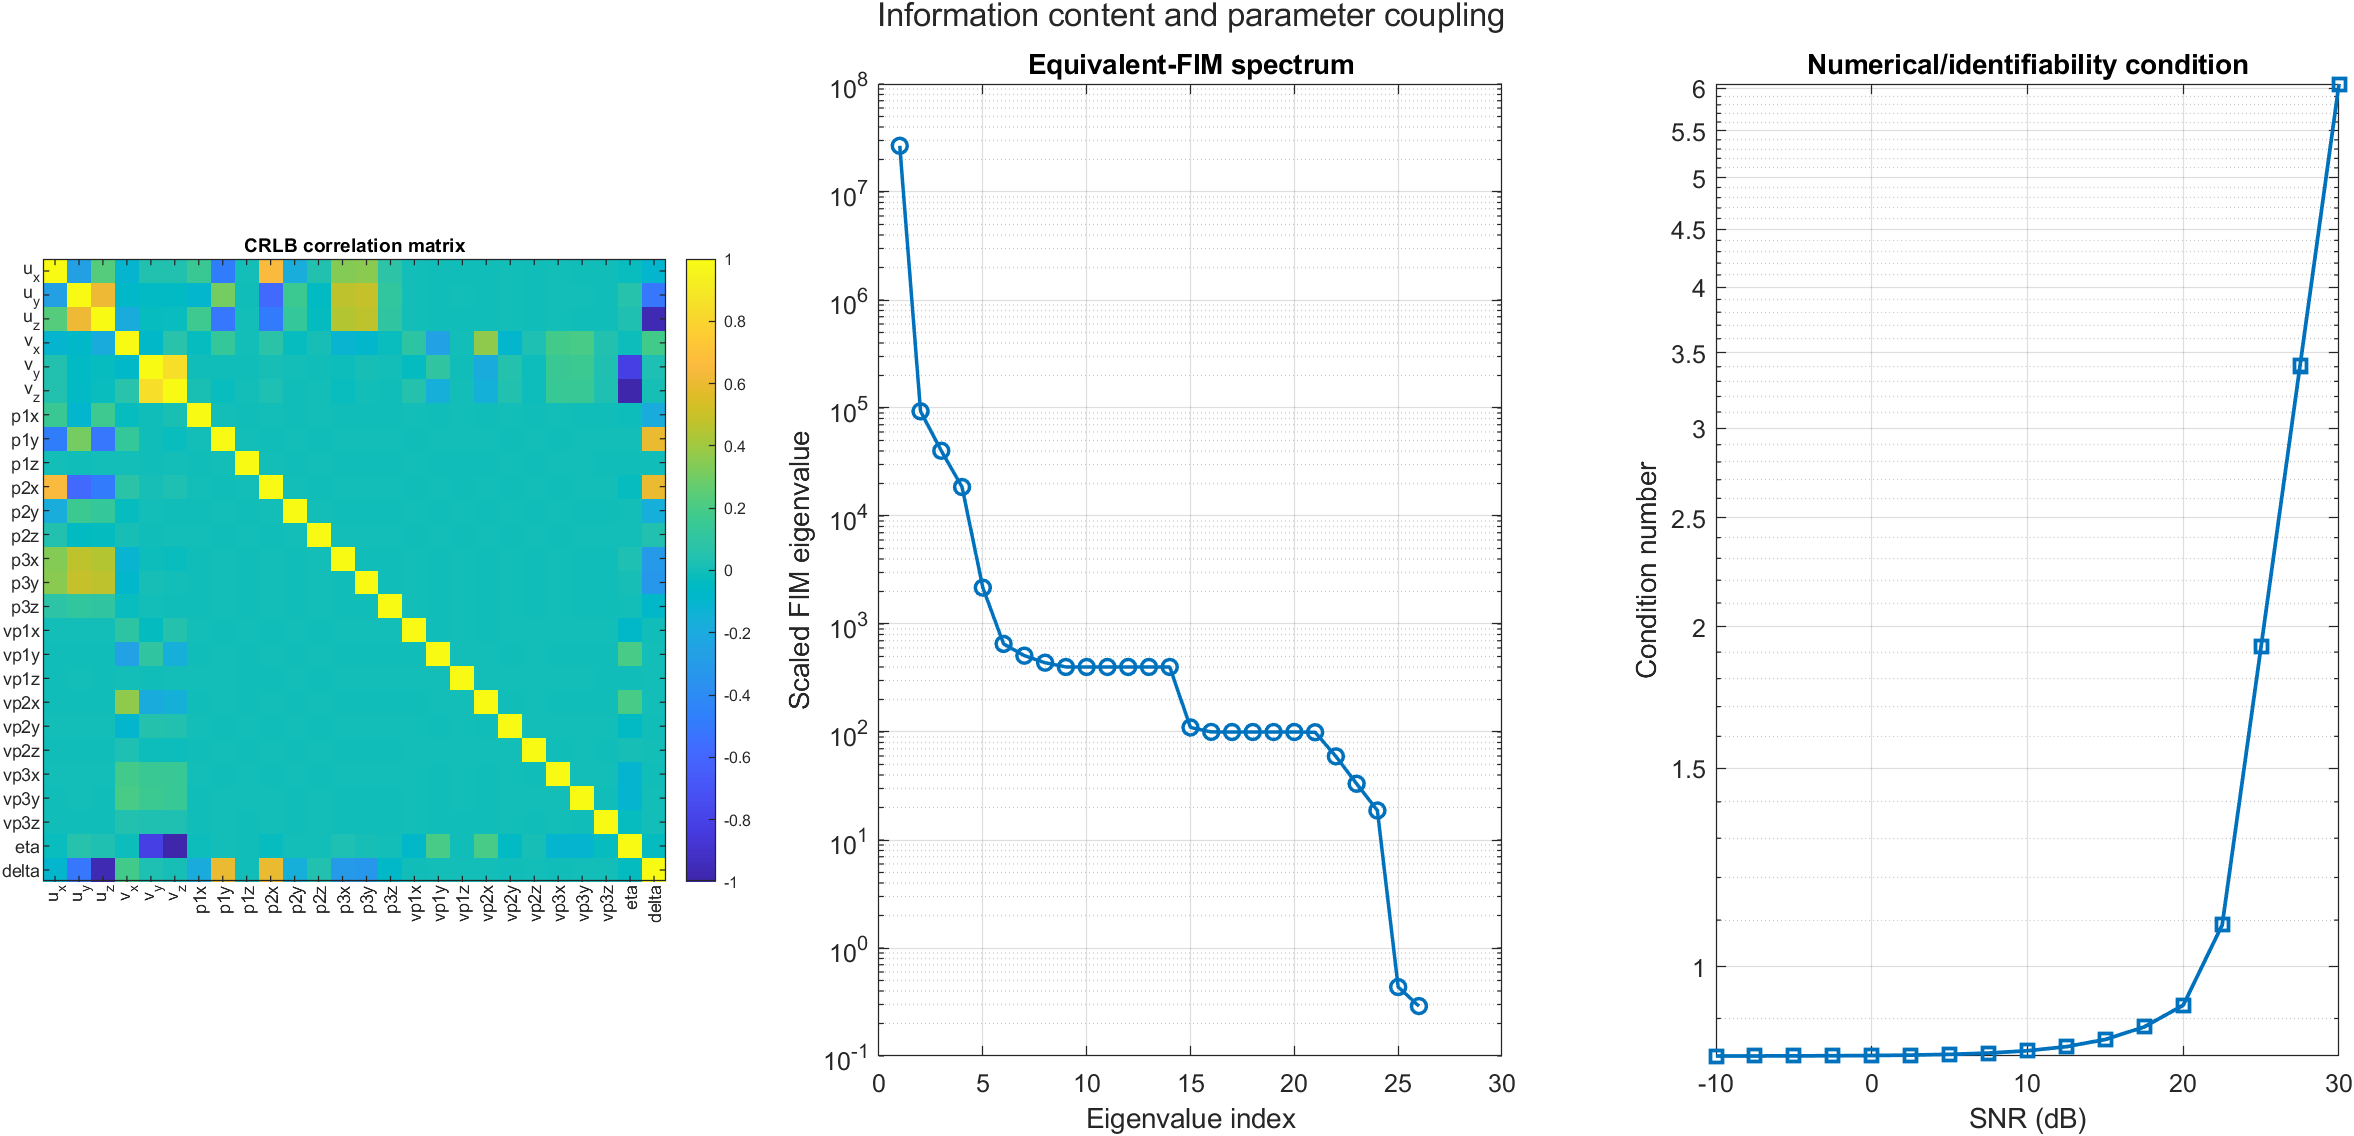
\includegraphics[width=0.85\linewidth]{07_fim_diagnostics.png}
\caption{Bound correlation matrix, FIM eigenvalue spectrum and identifiability indicators.}
\label{fig:fim}
\end{figure}

\paragraph{Sensitivity to the RIS prior.} The RIS position prior std was swept from 0.02 to 0.5~m, with the
velocity std scaled proportionally from 0.01 to 0.25~m/s (Table~\ref{tab:prior}, Fig.~\ref{fig:prior}). The UE
PEB grows almost linearly with $\sigma_p$, from 0.288~m to 5.822~m, and the VEB from 1.773 to 3.431~m/s. The RIS
uncertainty therefore enters the localization error budget directly: the prior is not just a regularization term,
its quality decides the final accuracy.

\begin{table}[H]
\centering
\caption{Sensitivity of the UE bounds to the RIS prior (\texttt{prior\_sensitivity.csv}).}
\label{tab:prior}
\begin{tabular}{rrrr}
\toprule
$\sigma_p$ (m) & $\sigma_v$ (m/s) & UE PEB (m) & UE VEB (m/s)\\
\midrule
0.02 & 0.010 & 0.288 & 1.773\\
0.05 & 0.025 & 0.606 & 1.793\\
0.10 & 0.050 & 1.176 & 1.864\\
0.20 & 0.100 & 2.334 & 2.124\\
0.50 & 0.250 & 5.822 & 3.431\\
\bottomrule
\end{tabular}
\end{table}

\begin{figure}[H]
\centering
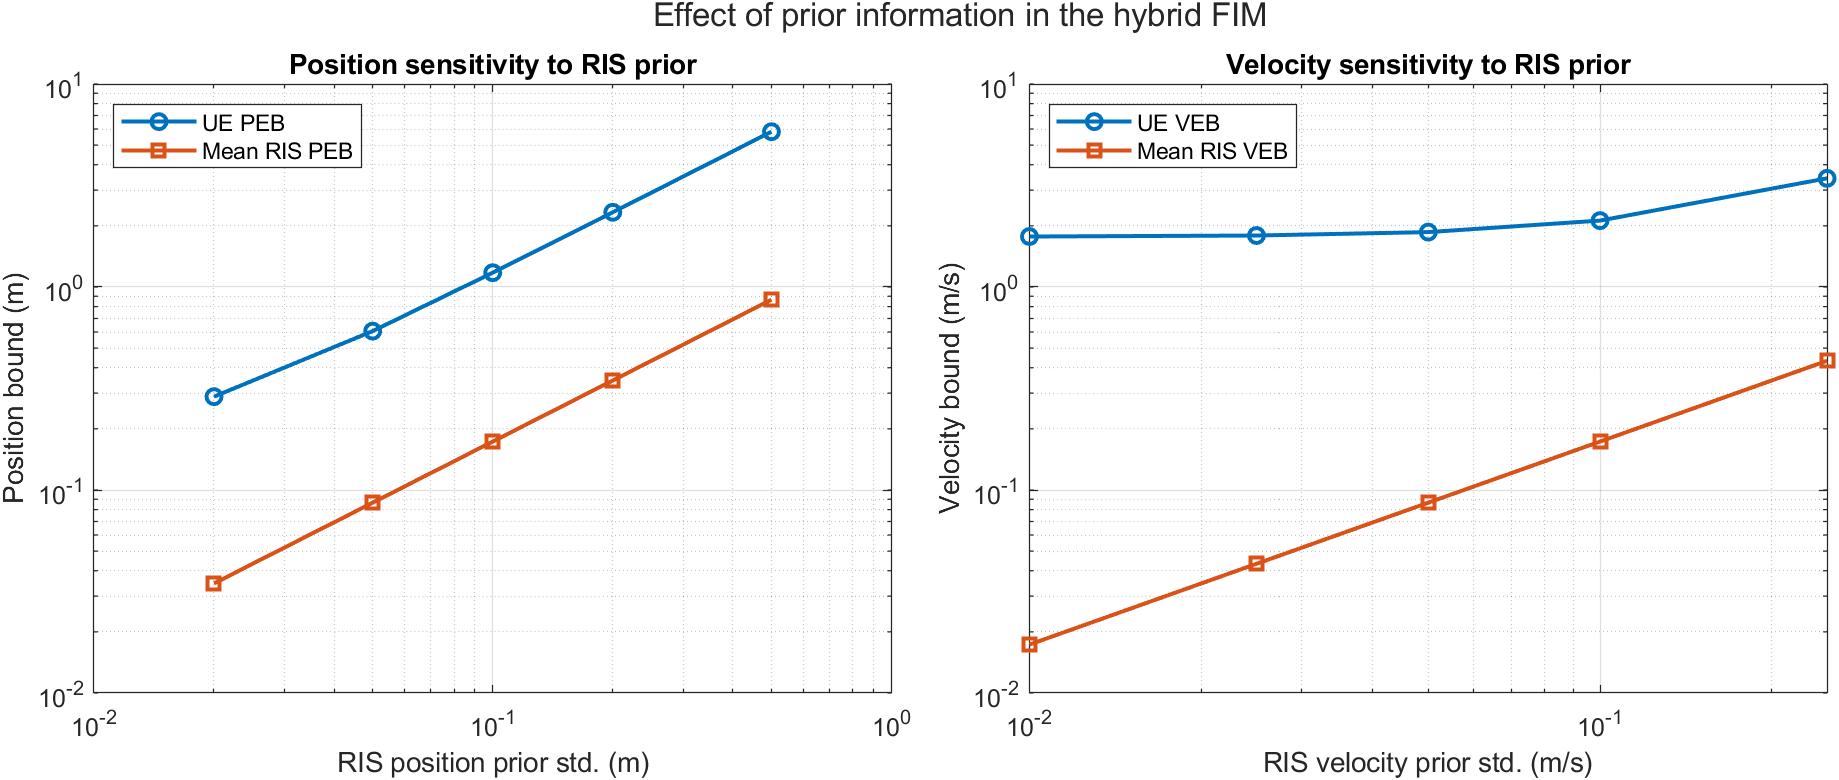
\includegraphics[width=0.7\linewidth]{08_prior_sensitivity.png}
\caption{Sensitivity of the UE position and velocity bounds to the RIS prior standard deviation.}
\label{fig:prior}
\end{figure}

\subsection{Hybrid MAP/ML estimator results}

\paragraph{Geometry and user parameters.} The prior mean of the RIS positions has small offsets of a few
centimetres from the true positions, so it is fairly accurate. In Fig.~\ref{fig:estgeom}, the final UE estimate
moves from the initial point towards the true position, while the estimated RIS positions stay close to the prior
mean --- consistent with the bound result that the prior dominates the RIS states. The data are used mainly to
improve the UE estimate rather than to move the RISs.

\begin{figure}[H]
\centering
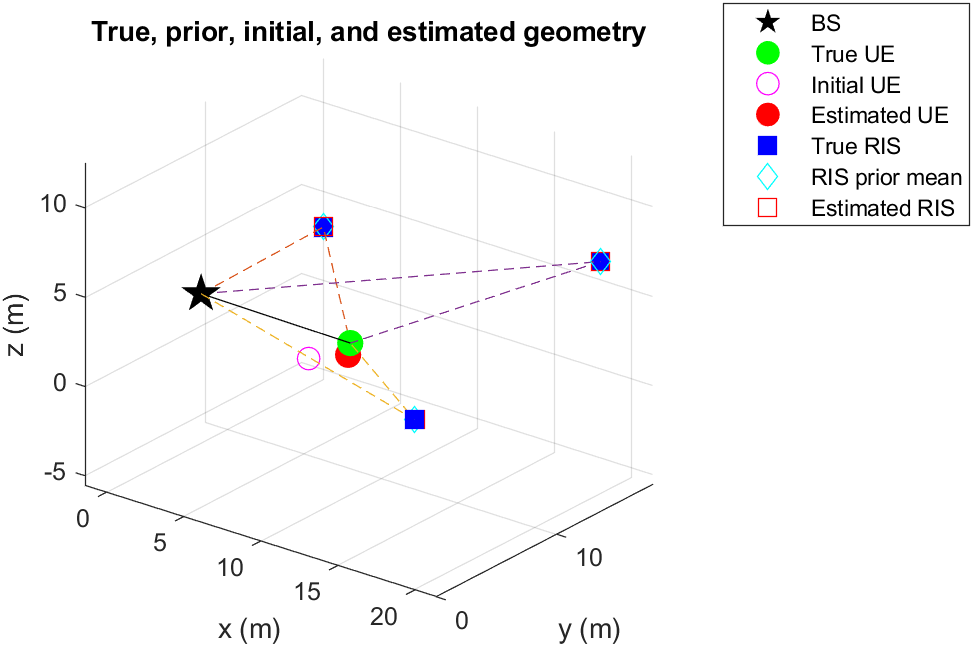
\includegraphics[width=0.62\linewidth]{geometry.png}
\caption{True geometry, prior mean, initial point and final estimate.}
\label{fig:estgeom}
\end{figure}

\begin{table}[H]
\centering
\caption{UE parameters in the estimator run (\texttt{physical\_parameters.csv}).}
\label{tab:ue}
\begin{tabular}{lrrrrr}
\toprule
Parameter & True & Initial & Estimate & Error & Local std bound\\
\midrule
$u_x$ (m) & 8.000 & 7.800 & 8.0185 & 0.0185 & 0.1373\\
$u_y$ (m) & 10.000 & 6.800 & 9.8000 & $-0.2000$ & 0.2194\\
$u_z$ (m) & 1.500 & 1.700 & 0.9162 & $-0.5838$ & 1.0483\\
$\dot u_x$ (m/s) & 1.200 & 1.000 & 1.3672 & 0.1672 & 0.3112\\
$\dot u_y$ (m/s) & $-0.400$ & $-0.300$ & $-0.4696$ & $-0.0696$ & 0.1906\\
$\dot u_z$ (m/s) & 0.100 & 0.000 & 0.3569 & 0.2569 & 0.8496\\
\bottomrule
\end{tabular}
\end{table}

The vector UE position error drops from 3.212~m at the initial point to 0.617~m, an improvement of about 80.8\%
(Table~\ref{tab:ue}). The $x$ component is the most accurate (0.0185~m error); the height error
($-0.5838$~m) contributes most of the final error, consistent with its large local bound (1.0483~m) and with the
weak vertical direction found in the bound analysis.

\paragraph{Active local bound.} The estimate of $u_y$ is exactly 9.8~m, i.e.\ on the upper edge of the local box
($6.8+3$~m), while the true value 10~m lies outside it. Part of this error is therefore caused by the choice of the
local search region, not only by noise or limited information.

The velocity error grows from about 0.245~m/s at the initial point to 0.314~m/s. This does not mean the estimator
fails: the bound describes average performance over many noise realizations and does not require every subset of
parameters to improve in a single run. It does, however, show that the velocity estimate needs a Monte Carlo
evaluation.

\paragraph{Synchronization initialization.} The grid search reduces the initial cost from 407\,890 to
106\,313, moving the starting point from $(\eta,\delta_c)=(1~\text{ppm},30~\text{ns})$ to $(2~\text{ppm},35~\text{ns})$
(Fig.~\ref{fig:sync}). The cost surface is elongated along $\delta_c$, so the clock offset is less separable at
this stage, while the cost changes faster along $\eta$ thanks to the time information from many snapshots. Local
optimization then gives $\hat\eta=1.999864$~ppm and $\hat\delta_c=40.4181$~ns, i.e.\ absolute errors of
0.000136~ppm and 0.418~ns.

\begin{figure}[H]
\centering
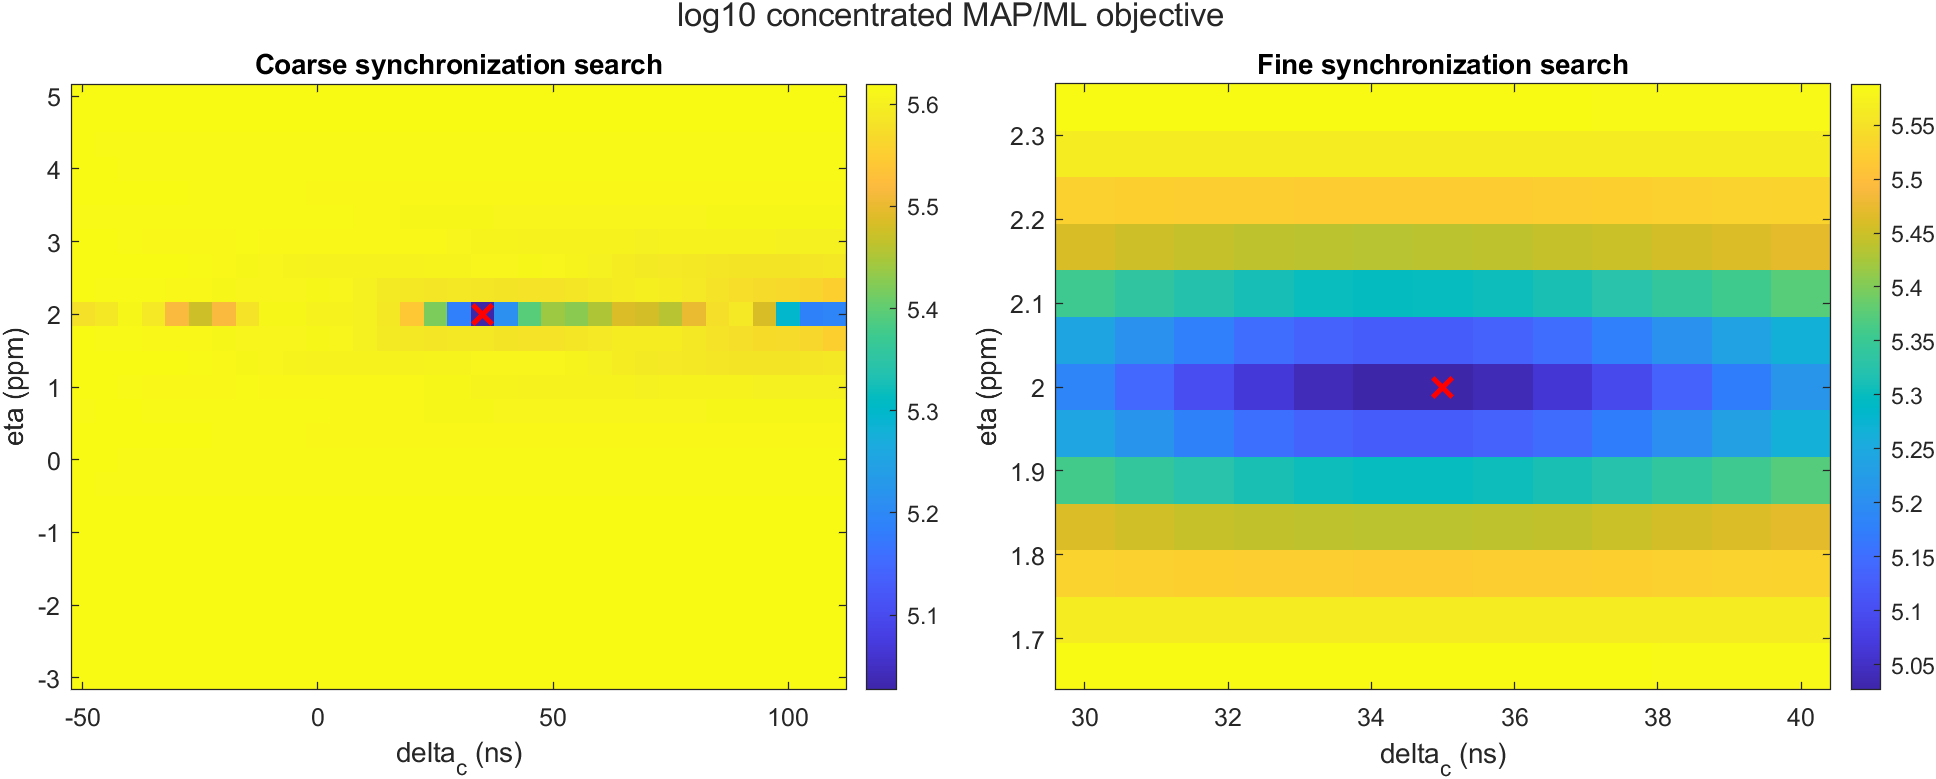
\includegraphics[width=0.8\linewidth]{sync_initialization.png}
\caption{Concentrated cost surface in the coarse and fine synchronization search.}
\label{fig:sync}
\end{figure}

\paragraph{Convergence, residual and channel gains.} All eight selected starts converge to almost the same final
cost (4123.258); the best start stopped after about 80 iterations with exit flag 2 (step size below tolerance,
constraints satisfied). The residual map shows no noticeable structure after the fit (Fig.~\ref{fig:diag}). The
data part of the cost is 4123.136 and the prior part only 0.1218, so the normalized residual is
$4123.136/4128=0.99882$, consistent with the assumed noise variance. Convergence of all starts to the same value
indicates a stable solution inside the chosen search region, though it does not prove global optimality.

\begin{figure}[H]
\centering
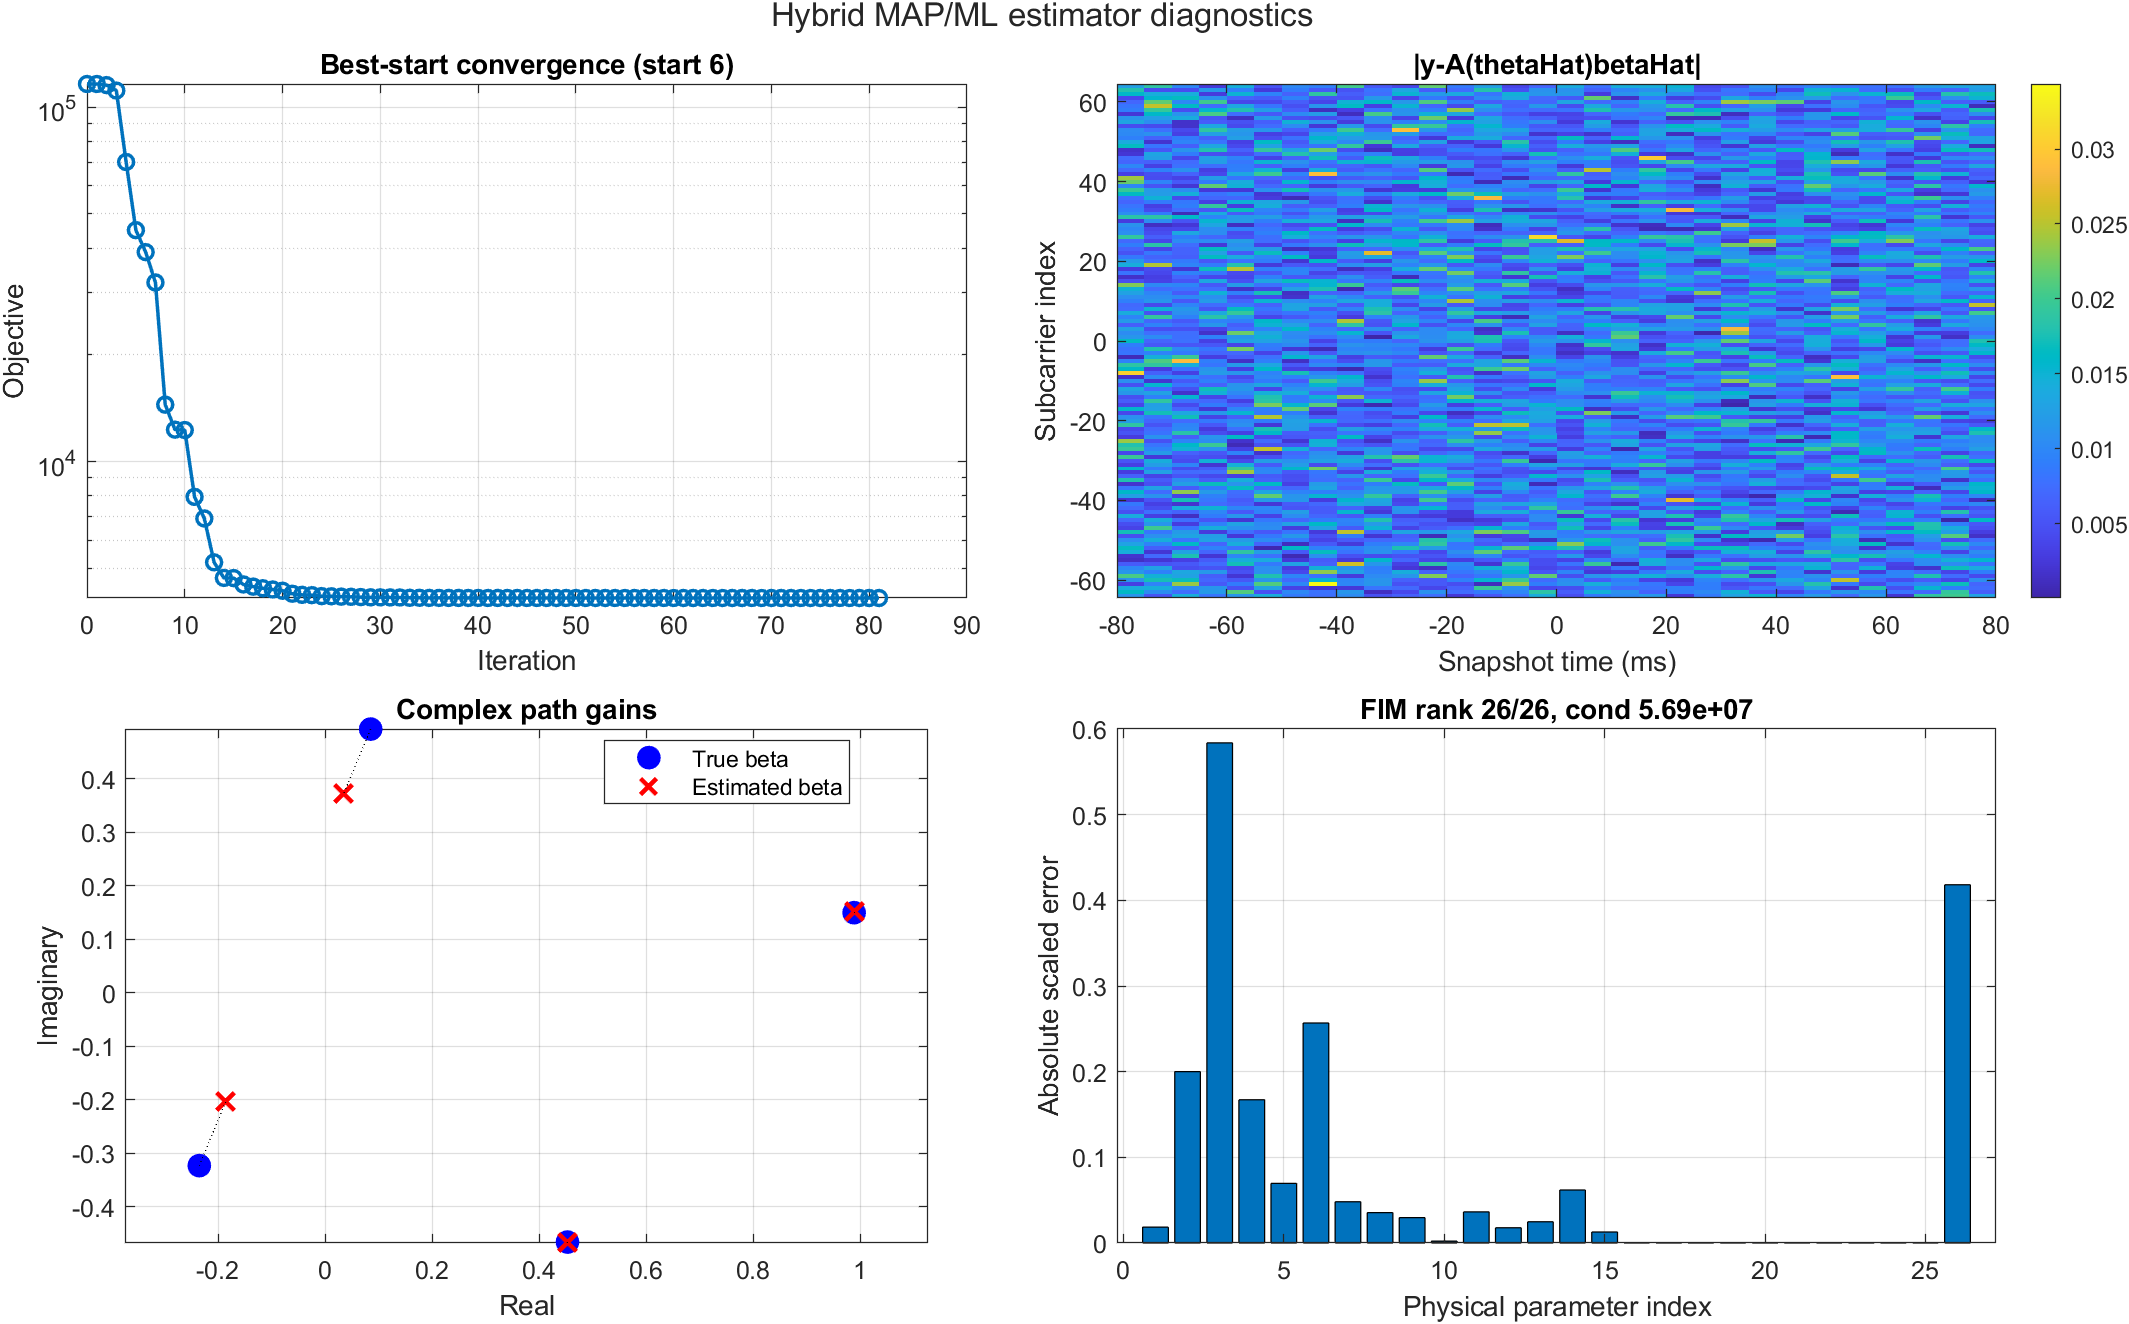
\includegraphics[width=0.95\linewidth]{diagnostics.png}
\caption{Estimator diagnostics: convergence of the best start, residual map, complex path gains and absolute
scaled error of the physical parameters.}
\label{fig:diag}
\end{figure}

\begin{table}[H]
\centering
\caption{True and estimated complex path gains (\texttt{channel\_parameters.csv}).}
\label{tab:beta}
\begin{tabular}{crrr}
\toprule
$k$ & True $\beta_k$ & Estimated $\hat\beta_k$ & Absolute error\\
\midrule
0 & $0.98877+j0.14944$ & $0.98984+j0.15166$ & 0.00247\\
1 & $0.45286-j0.46628$ & $0.45206-j0.46788$ & 0.00179\\
2 & $0.08498+j0.49272$ & $0.03470+j0.37246$ & 0.13036\\
3 & $-0.23540-j0.32340$ & $-0.18601-j0.20389$ & 0.12932\\
\bottomrule
\end{tabular}
\end{table}

The gains of the first two paths are estimated very accurately, while paths 2 and 3 have absolute errors of about
0.13 (Table~\ref{tab:beta}). This agrees with the information analysis (some gain components carry less
information) and with the coupling between path gains, geometry and synchronization, through which part of the
geometric error can leak into the gains. At the estimate, the local equivalent FIM has rank 26/26 and condition
number $5.69\times10^{7}$: locally identifiable, but with very uneven information across directions.

\subsection{Summary of the numerical analysis}
\begin{enumerate}
\item The quality of the RIS prior directly limits UE localization: increasing the RIS position uncertainty can
multiply the UE PEB, so the accuracy of the RIS geometry is part of the fundamental localization limit.
\item With three RISs and 32 snapshots the physical FIM is full rank, but its condition number is of order
$10^{7}$--$10^{8}$; the vertical component of UE position and velocity is one of the weakest directions.
\item Analytic removal of the gains, grid initialization of the synchronization parameters and multi-start
optimization improve the solution markedly over the initial point (3.212~m $\to$ 0.617~m), and all eight starts
reach practically the same cost.
\item The local bound on $u_y$ was active in the final solution, so the local search region --- especially along
$y$ --- should be enlarged, or the problem re-solved with a larger region whenever a bound becomes active.
\item The estimator results come from a single noise realization; a proper comparison with the bound requires
identical scenarios and Monte Carlo RMSE at several SNR values.
\end{enumerate}

%======================================================================
\section{Conclusions and Future Work}
%======================================================================

\subsection{Conclusions}
This project studied the localization and synchronization of a mobile UE aided by RISs whose geometry is
uncertain. Instead of treating this uncertainty as an external disturbance, it was built into the statistical
model, the bound and the estimator: UE, synchronization and channel parameters were modelled as deterministic
unknowns, and the RIS states as random parameters with a prior. The OFDM model showed that geometric delay,
motion, frequency error and clock offset act jointly on the phase, so subcarrier (frequency) diversity and snapshot
(time) diversity are complementary sources of information. The hybrid FIM combined data and prior information; the
channel gains were removed with a Schur complement while the uncertain RIS states were kept, preserving the effect
of their uncertainty in the final bound. At 20~dB, the bound gave a UE PEB of 1.176~m and VEB of 1.864~m/s, with the
vertical axis weakest. The prior sensitivity study showed that the quality of the RIS map is part of the error
budget: in practice, better calibration and RIS localization can matter as much as more power or more observations.
The hybrid MAP/ML estimator, with variable projection, coarse-to-fine synchronization search, multi-start and
constrained local optimization, reduced the UE position error from 3.212~m to 0.617~m with a normalized residual
close to one. These results describe the behaviour, sensitivities and practicality of the method rather than a
final claim that the estimator attains the bound.

\subsection{Limitations}
\begin{enumerate}
\item \textbf{Constant-velocity motion} --- not valid under acceleration or sudden manoeuvres.
\item \textbf{ICI neglected} --- may miss part of the data structure for large frequency errors, strong Doppler or
fast-varying channels.
\item \textbf{Constant channel gains over the block} --- real gains may change with motion, blockage or RIS
reconfiguration.
\item \textbf{Different geometries in the two output sets} --- direct comparison of estimator error with the other
scenario's bound is not valid.
\item \textbf{Single noise realization} --- not enough for statistical conclusions; RMSE over many realizations is
needed.
\item \textbf{Local optimization and search bounds} --- no guarantee of a global minimum, and the active local
bound on $u_y$ is partly responsible for its error.
\item \textbf{Limited geometries} --- rank, condition number and bounds can change considerably with BS, UE and RIS
placement and with the number of paths.
\end{enumerate}

\subsection{Future work}
\begin{enumerate}
\item Fully align the bound and estimator scenarios and run Monte Carlo trials at several SNRs to compare RMSE
directly with the CRLB.
\item Extend the motion model with acceleration (re-deriving geometric derivatives and re-checking
identifiability).
\item Model ICI explicitly and determine the range of speeds and frequency errors in which the current
approximation holds.
\item Use a time-varying channel model (piecewise-constant, stochastic or low-dimensional in time) for
$\vect{\beta}$.
\item Study more RISs and more diverse geometries, and design RIS placement using PEB, VEB, the smallest
eigenvalue or the condition number.
\item Extend to multiple users (shared RISs, interference, pilot allocation, and joint use of multi-user data for
RIS calibration).
\item Adapt the local search region automatically: re-solve with a larger region when a local bound becomes
active, and compare with more global strategies or geometry-based initialization.
\item Study robustness to model errors in $\sigma^2$, $\sigma_p$, $\sigma_v$ and to unmodelled paths.
\end{enumerate}

\appendix
\section{Parameter Ordering and Output Files}

\begin{table}[H]
\centering
\caption{Indices of the physical parameters in $\vect{\theta}$ for $K=3$.}
\begin{tabular}{cll}
\toprule
Index & Parameter & Unit\\
\midrule
1--3 & UE initial position $\vect{u}_0$ & m\\
4--6 & UE velocity $\udot$ & m/s\\
7--9, 10--12, 13--15 & RIS 1, 2, 3 positions $\vect{p}_{k,0}$ & m\\
16--18, 19--21, 22--24 & RIS 1, 2, 3 velocities $\pdot_k$ & m/s\\
25 & relative frequency error $\eta$ & --\\
26 & clock offset $\delta_c$ & s\\
\midrule
27--30 & $\Re\{\beta_0\},\dots,\Re\{\beta_3\}$ & --\\
31--34 & $\Im\{\beta_0\},\dots,\Im\{\beta_3\}$ & --\\
\bottomrule
\end{tabular}
\end{table}

\begin{table}[H]
\centering
\caption{CSV outputs of the two packages.}
\small
\begin{tabular}{ll}
\toprule
File & Content\\
\midrule
\multicolumn{2}{l}{\textit{Bound package (\texttt{crlb/crlb\_results/})}}\\
\texttt{summary\_bounds.csv} & aggregate UE, RIS and synchronization bounds at the default SNR\\
\texttt{all\_parameter\_bounds.csv} & variance and std lower bound of each of the 34 parameters\\
\texttt{snr\_sweep\_bounds.csv} & bounds over $-10$ to $30$ dB\\
\texttt{prior\_sensitivity.csv} & PEB and VEB versus $\sigma_p$ and $\sigma_v$\\
\midrule
\multicolumn{2}{l}{\textit{Estimator package (\texttt{estimator/hybrid\_map\_results/})}}\\
\texttt{summary.csv} & aggregate errors, cost components, rank and condition number\\
\texttt{physical\_parameters.csv} & true, initial, estimated value, error and local bound per parameter\\
\texttt{channel\_parameters.csv} & true and estimated complex path gains\\
\texttt{multi\_start\_summary.csv} & initial and final cost and exit flag of each start\\
\texttt{sync\_initialization.csv} & result of the grid search over $\eta$ and $\delta_c$\\
\bottomrule
\end{tabular}
\end{table}

\begin{thebibliography}{9}
\bibitem{kay1993} S.~M.~Kay, \emph{Fundamentals of Statistical Signal Processing, Volume I: Estimation Theory}.
Prentice Hall, 1993.
\bibitem{vantrees2001} H.~L.~Van~Trees, \emph{Detection, Estimation, and Modulation Theory, Part I}, 2nd ed.
Wiley, 2001.
\bibitem{golub1973} G.~H.~Golub and V.~Pereyra, ``The differentiation of pseudo-inverses and nonlinear least
squares problems whose variables separate,'' \emph{SIAM Journal on Numerical Analysis}, vol.~10, no.~2,
pp.~413--432, 1973.
\bibitem{wymeersch2020} H.~Wymeersch and B.~Denis, ``Beyond 5G wireless localization with reconfigurable
intelligent surfaces,'' in \emph{Proc.\ IEEE International Conference on Communications (ICC)}, 2020.
\bibitem{stoica2005} P.~Stoica and R.~Moses, \emph{Spectral Analysis of Signals}. Prentice Hall, 2005.
\end{thebibliography}

\end{document}
